% !TeX root = ../../../main.tex
\subsection{Semi-Synthetic Datasets: Setup and Additional Results} 
\label{ch04:app:more-semi-syn-data-setup-result}

\ChFourHeadingOnly
\subsubsection{Semi-synthetic datasets setup}
To complement synthetic benchmarks and real-world case studies, we construct semi-synthetic datasets that pair real covariates with simulated treatment assignment and survival outcomes.
This strategy preserves realistic covariate distributions and correlations while enabling controlled evaluation against known ground-truth CATEs.
We consider two covariate sources: the ACTG HIV trial and MIMIC-IV ICU records.
Table~\ref{ch04:tab:semi-syn-dataset-summary} summarizes dataset sizes, covariate counts, treatment and censoring rates, and whether the treatment-assignment and event-time mechanisms depend on covariates through linear versus non-linear functions; full generative details are provided in Appendix~\ref{ch04:app:actg-semi-dataset} and~\ref{ch04:app:mimic-suite}.
Figure~\ref{ch04:fig:semi-syn-km-curves} shows Kaplan--Meier curves for event and censoring in the treatment and control groups for each semi-synthetic dataset.


% !TeX root = ../../../main.tex
\begin{table}[htbp]
\ChFourFloatContents{ch04:tab:semi-syn-dataset-summary}{\caption{Semi-synthetic datasets overview. The last two columns summarize how treatment assignment and event-time generation depend on covariates. \texttt{linear} indicates dependence through a linear predictor with no quadratic or interaction terms; \texttt{non-linear} includes quadratic and/or interaction terms. \texttt{independent} indicates covariate-independent treatment assignment.}}{
    
     
    \centering
    \setlength{\tabcolsep}{5pt}
    \begin{adjustbox}{max width = \textwidth}
    \begin{tabular}{@{}lcccccc@{}}
        \toprule
        & \makecell{\textbf{Data}\\\textbf{size}} 
        & \makecell{\textbf{No.}\\\textbf{covariates}} 
        & \makecell{\textbf{Treatment}\\\textbf{rate}} 
        & \makecell{\textbf{Censoring.}\\\textbf{rate}} 
        & \makecell{\textbf{Treatment assignment}\\\textbf{mechanism}} 
        & \makecell{\textbf{Event time}\\\textbf{mechanism}} \\
        \midrule
        ACTG & 2,139 & 23 & 56.15\% & 51.19\% & \texttt{linear} & \texttt{non-linear} \\ 
        \addlinespace
        MIMIC-$i$ & 25,170 & 36 & 49.92\% & 88.49\% & \texttt{independent} & \texttt{linear} \\ 
        MIMIC-$ii$ & 25,170 & 36 & 49.92\% & 81.65\% & \texttt{independent} & \texttt{linear} \\ 
        MIMIC-$iii$ & 25,170 & 36 & 49.92\% & 74.10\% & \texttt{independent} & \texttt{linear} \\ 
        MIMIC-$iv$ & 25,170 & 36 & 49.92\% & 66.34\% & \texttt{independent} & \texttt{linear} \\ 
        MIMIC-$v$ & 25,170 & 36 & 49.92\% & 53.35\% & \texttt{independent} & \texttt{linear} \\ 
        \addlinespace
        MIMIC-$vi$ & 25,170 & 36 & 53.54\% & 53.07\% & \texttt{linear} & \texttt{linear} \\ 
        MIMIC-$vii$ & 25,170 & 36 & 54.26\% & 52.66\% & \texttt{linear} & \texttt{non-linear} \\ 
        MIMIC-$viii$ & 25,170 & 36 & 50.94\% & 53.26\% & \texttt{non-linear} & \texttt{linear} \\ 
        MIMIC-$ix$ & 25,170 & 36 & 51.47\% & 52.82\% & \texttt{non-linear} & \texttt{non-linear} \\ 
        \bottomrule
    \end{tabular}
    \end{adjustbox}
    \par
}
\end{table}



% !TeX root = ../../../main.tex
\begin{figure}[htbp]
\ChFourFloatContents{ch04:fig:semi-syn-km-curves}{\caption{(Semi-synthetic datasets) Kaplan-Meier curves. Solid lines show event-time survival under control (blue) and treatment (orange); dotted lines show censoring-time survival for each arm. Each panel reports the empirical censoring rate $c$ and treatment probability $p$.}}{
  \centering
  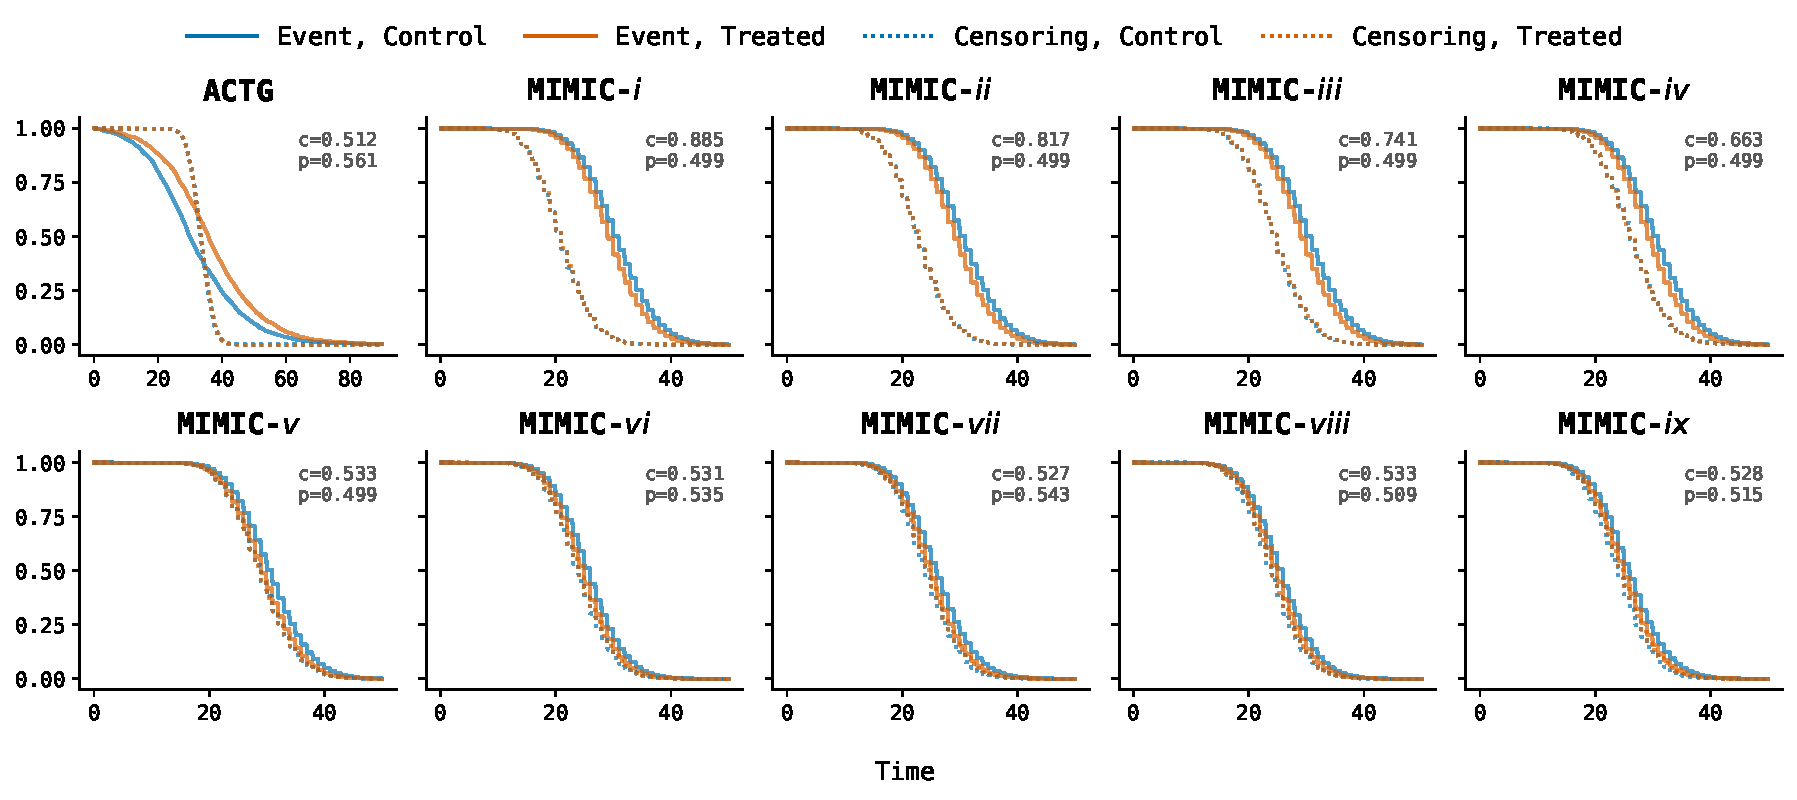
\includegraphics[width=0.98\linewidth]{Appendices/appendix-ch04/images/figure_results_updated/semi-syn-km-curves.pdf} 
   
}
\end{figure}




\subsubsection{ACTG semi-synthetic dataset} \label{ch04:app:actg-semi-dataset}
The ACTG semi-synthetic dataset is derived from the ACTG 175 HIV clinical trial \citep{hammer1996atrial}, which contains 23 baseline covariates.
Following the construction procedure of \citet{chapfuwa2021enabling}, we simulate covariate-dependent treatment assignment and generate event times from a Gompertz--Cox model with an AFT-style censoring mechanism.
This dataset exhibits realistic treatment imbalance and moderate censoring ($\sim$51\%), providing a clinically grounded benchmark with preserved trial covariate structure.

More concretely, following \citet{chapfuwa2021enabling}, we generate: 
$$X = \text{ACTG covariates}$$
$$P(A=1|X=x) = \frac{1}{b} \times \left(a + \sigma\left( \eta ({\rm AGE} - \mu_{\rm AGE} + {\rm CD40} - \mu_{\rm CD40}) \right) \right)$$
$$ U  \sim {\rm Uniform} (0, 1 )$$
$$T_A  =  \frac{1}{\alpha_A} \log \left[1 - \frac{\alpha_A \log U}{ \lambda_A  \exp\left( x ^T  \beta_A\right)  }  \right]$$
$$\log C  \sim {\rm Normal} (\mu_c, \sigma_c^2)$$
$$Y = \min(T_A, C)$$
where $\sigma(\cdot)$ is the sigmoid function, $\{ \beta_A, \alpha_A, \lambda_A, b, a, \eta, \mu_c, \sigma_c \}$ are hyper-parameters taken to be the same as described at \url{https://github.com/paidamoyo/counterfactual_survival_analysis} and $\{\mu_{\rm AGE},  \mu_{\rm CD40}\}$ are the means for age and CD40 respectively.


\subsubsection{MIMIC semi-synthetic datasets}
\label{ch04:app:mimic-suite}
{\raggedright We construct a suite of nine semi-synthetic datasets derived from MIMIC-IV ICU records~\citep{johnson2023mimic}. All variants share the same covariates and sample size, and differ only in the treatment-assignment and event/censoring mechanisms. The suite is organized into two complementary subsets: (1) \emph{independent assignment with varying censoring severity} (MIMIC-$i$--$v$), which isolates robustness to censoring under randomized treatment; and (2) \emph{confounded assignment with varying functional form} (MIMIC-$vi$--$ix$), which evaluates robustness to observed confounding and to non-linear (interaction-based) event and censoring mechanisms while keeping covariates fixed.\par}


We extract 36 covariates spanning laboratory test abnormalities (e.g., creatinine, glucose, hemoglobin), demographic features (e.g., age, sex, race, marital status), and admission descriptors (e.g., admission type, recurrent admissions, night admission).
Table~\ref{ch04:tab:mimic-covariates} summarizes covariate statistics; Table~\ref{ch04:tab:mimic-demographics} reports demographic and categorical distributions; and Figure~\ref{ch04:fig:mimic_corr} shows correlations among covariates.



% !TeX root = ../../../main.tex
\begin{table}[htbp]
\ChFourFloatContents{ch04:tab:mimic-covariates}{\caption{Summary statistics of MIMIC semi-synthetic covariates. Reported values are mean $\pm$ standard deviation. 
    Physiological covariates are coded as indicators for abnormal values where mean reflects prevalence of abnormality.}}{
    

    
    \centering
    \begin{adjustbox}{max width = 0.7\textwidth}
    \begin{tabular}{
        l
        >{\centering\arraybackslash}p{0.18\textwidth}
        l
        >{\centering\arraybackslash}p{0.18\textwidth}
    }
    
    \toprule
    \textbf{Covariate} & Mean $\pm$ Std & \textbf{Covariate} & Mean $\pm$ Std \\
    \midrule
    Sodium & 0.12 $\pm$ 0.32 & Admission age & 61.39 $\pm$ 17.97 \\
    Potassium & 0.08 $\pm$ 0.28 & Sex:Male & 0.51 $\pm$ 0.50 \\
    Chloride & 0.19 $\pm$ 0.39 & Race:White & 0.70 $\pm$ 0.46 \\
    Bicarbonate & 0.24 $\pm$ 0.43 & Race:Black & 0.14 $\pm$ 0.35 \\
    Anion gap & 0.09 $\pm$ 0.29 & Race:Hispanic & 0.05 $\pm$ 0.22 \\
    Creatinine & 0.28 $\pm$ 0.45 & Race:Other & 0.07 $\pm$ 0.25 \\
    Urea nitrogen & 0.40 $\pm$ 0.49 & Insurance:Medicare & 0.42 $\pm$ 0.49 \\
    Glucose & 0.65 $\pm$ 0.48 & Insurance:Other & 0.52 $\pm$ 0.50 \\
    Calcium total & 0.29 $\pm$ 0.45 & Marital status:Married & 0.45 $\pm$ 0.50 \\
    Magnesium & 0.09 $\pm$ 0.28 & Marital status:Single & 0.33 $\pm$ 0.47 \\
    Phosphate & 0.28 $\pm$ 0.45 & Marital status:Widowed & 0.14 $\pm$ 0.34 \\
    Hemoglobin & 0.73 $\pm$ 0.44 & Direct emergency:Yes & 0.11 $\pm$ 0.31 \\
    Hematocrit & 0.69 $\pm$ 0.46 & Night admission:Yes & 0.54 $\pm$ 0.50 \\
    MCV & 0.20 $\pm$ 0.40 & \makecell{Previous admission\\this month: Yes} & 0.08 $\pm$ 0.27 \\
    MCH & 0.26 $\pm$ 0.44 & Admissions number:2 & 0.16 $\pm$ 0.37 \\
    MCHC & 0.31 $\pm$ 0.46 & Admissions number:3+ & 0.22 $\pm$ 0.42 \\
    Platelet count & 0.29 $\pm$ 0.45 & & \\
    RDW & 0.29 $\pm$ 0.45 & & \\
    White blood cells & 0.40 $\pm$ 0.49 & & \\
    Red blood cells & 0.76 $\pm$ 0.43 & & \\
    \bottomrule
    \end{tabular}
    \end{adjustbox}
}
\end{table}




% !TeX root = ../../../main.tex
\begin{table}[htbp]
\ChFourFloatContents{ch04:tab:mimic-demographics}{\caption{Demographic and categorical distributions in MIMIC semi-synthetic datasets. Reported values are proportions.}}{
  
  
  \centering \small
  \begin{minipage}[t]{0.48\textwidth}
    \centering
    \textbf{Demographics}\par
    \begin{tabular}{lc}
      \toprule
      Variable & Proportion \\
      \midrule
      \textbf{Sex} & \\
      Male   & 0.512 \\
      Female & 0.488 \\
      \addlinespace
      \textbf{Race} & \\
      White    & 0.699 \\
      Black    & 0.141 \\
      Other    & 0.066 \\
      Hispanic & 0.053 \\
      Asian    & 0.041 \\
      \addlinespace
      \textbf{Insurance} & \\
      Other    & 0.522 \\
      Medicare & 0.421 \\
      Medicaid & 0.057 \\
      \addlinespace
      \textbf{Marital status} & \\
      Married  & 0.449 \\
      Single   & 0.334 \\
      Widowed  & 0.136 \\
      Divorced & 0.081 \\
      \bottomrule
    \end{tabular}
  \end{minipage}
  \hfill
  \begin{minipage}[t]{0.48\textwidth}
    \centering
    \textbf{Admission-related}\par
    \begin{tabular}{lc}
      \toprule
      Variable & Proportion \\
      \midrule
      \textbf{Direct emergency} & \\
      Yes & 0.110 \\
      No  & 0.890 \\
      \addlinespace
      \textbf{Night admission} & \\
      Yes & 0.539 \\
      No  & 0.461 \\
      \addlinespace
      \textbf{\makecell{Previous admission\\this month}} & \\
      Yes & 0.081 \\
      No  & 0.919 \\
      \addlinespace
      \textbf{Admissions number} & \\
      1   & 0.615 \\
      2   & 0.164 \\
      3+  & 0.222 \\
      \bottomrule
    \end{tabular}
  \end{minipage}
}
\end{table}



% !TeX root = ../../../main.tex
\begin{figure}[htbp]
\ChFourFloatContents{ch04:fig:mimic_corr}{\caption{Correlation heatmap of the 36 semi-synthetic MIMIC covariates. Variables include demographic features, admission descriptors, insurance and marital status indicators, and laboratory measurements. Most correlations are weak to moderate, with stronger dependencies visible among related laboratory values (e.g., hematocrit, hemoglobin, and red blood cell count).}}{
  \centering
  
  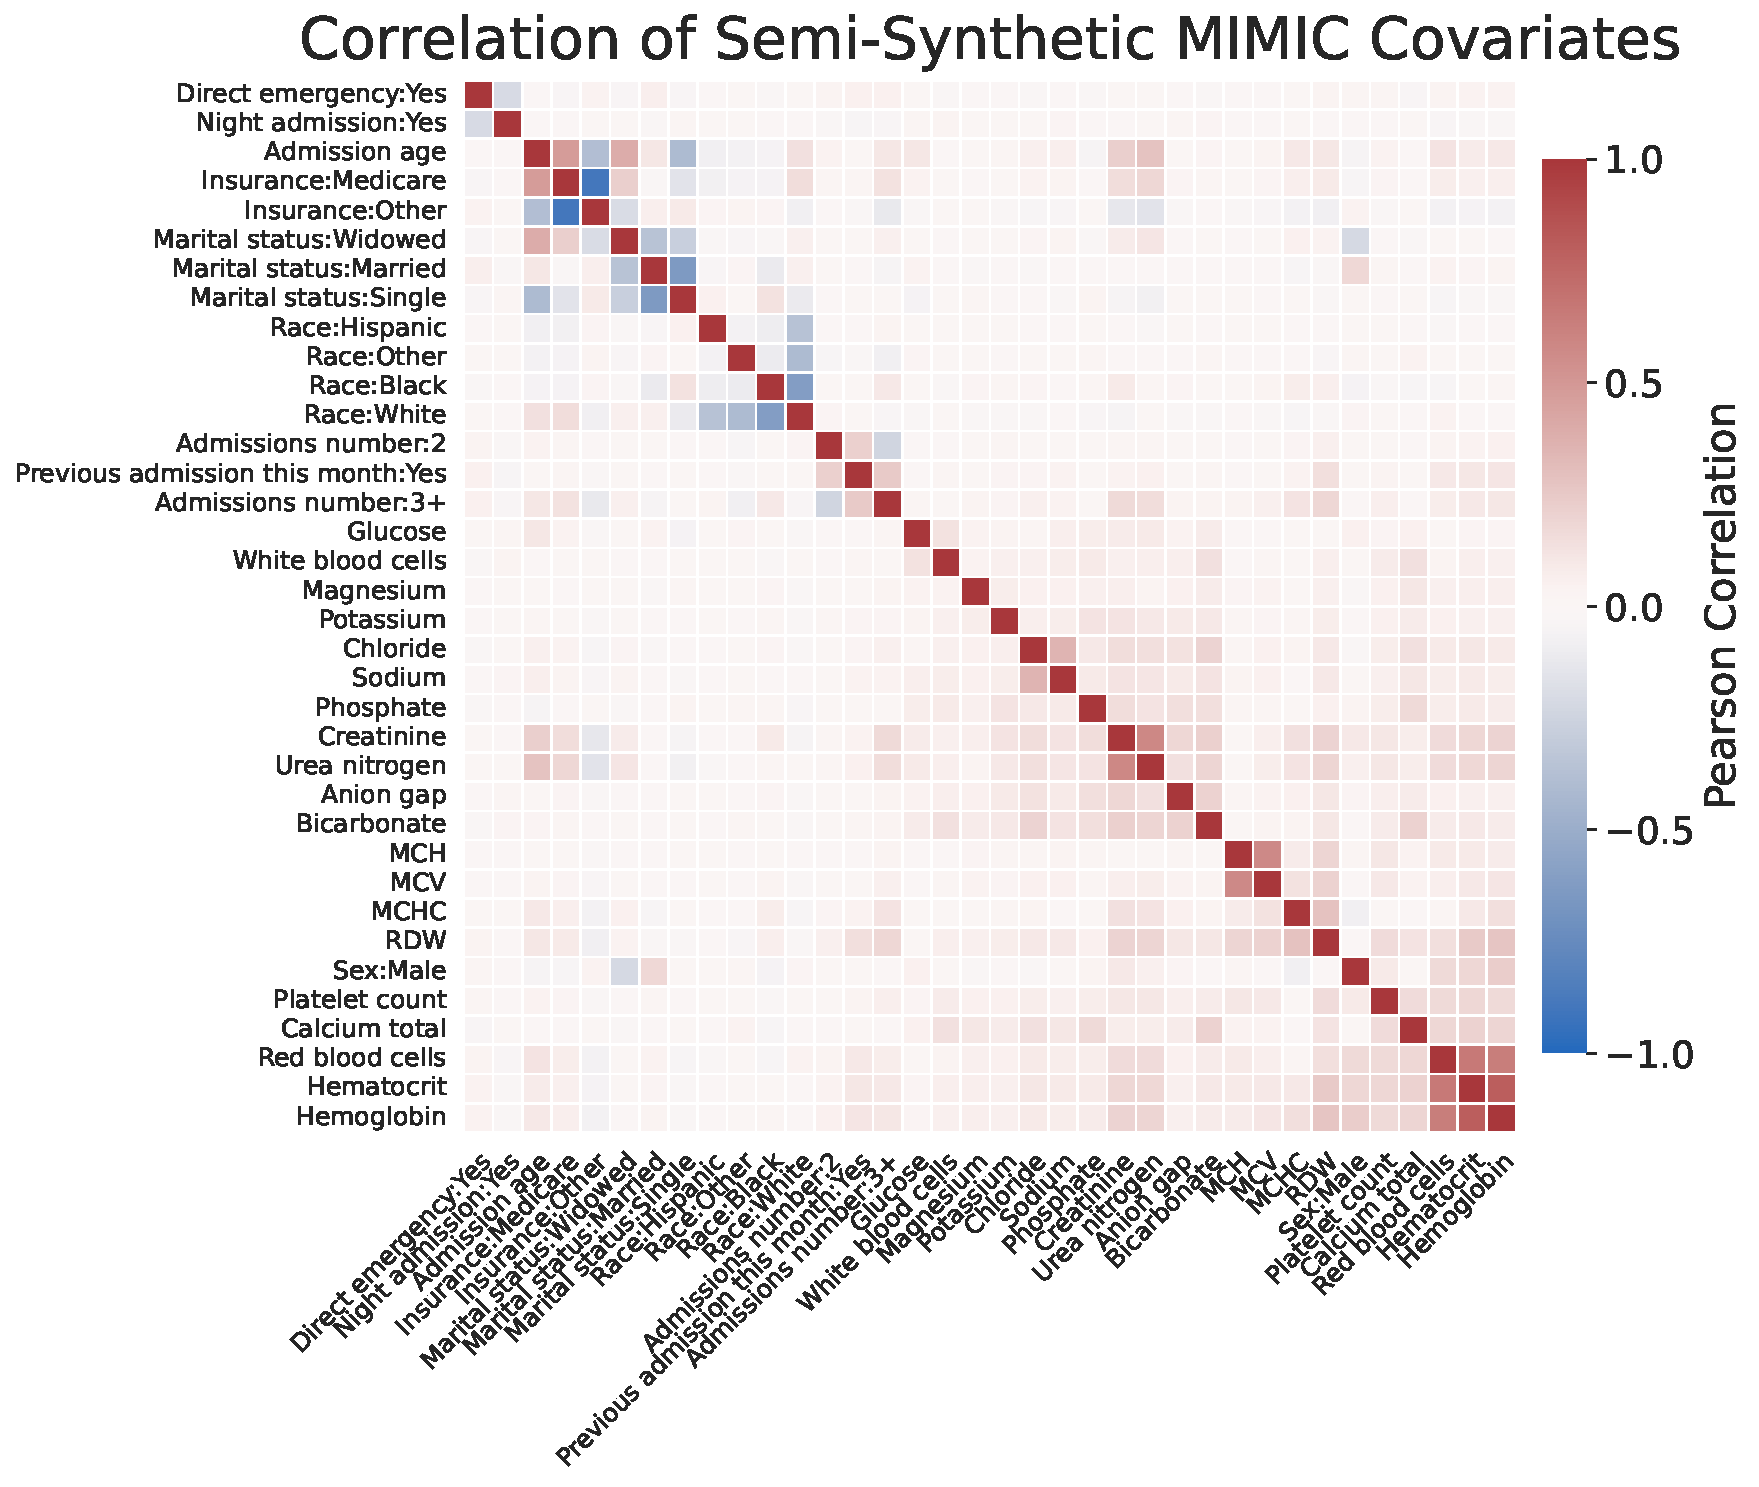
\includegraphics[width=.8\linewidth]{Appendices/appendix-ch04/images/figure_results_updated/corr_heatmap_mimic.pdf}
   
  
}
\end{figure}


We now introduce some shared notation in all of the MIMIC semi-synthetic datasets.
Let $X_{1:5}$ denote the first five binary covariates corresponding to abnormal laboratory values
(\textit{Anion gap}, \textit{Bicarbonate}, \textit{Calcium total}, \textit{Chloride}, \textit{Creatinine}),
and let $X_{36}$ denote the standardized \textit{Admission age}.
We define the abnormal-lab burden as
\[
S = \sum_{j=1}^{5} X_j.
\]
Across all MIMIC variants, we generate potential event times $T(0),T(1)$ and a censoring time $C$, and observe
\[
T = W T(1) + (1-W)T(0),\quad Y=\min(T,C),\quad \delta=\ChFourInd\{T\le C\}.
\]


\paragraph{Independent-assignment, varying censoring (MIMIC-$i$--$v$)}
\label{ch04:app:mimic-i-v}
This subset follows the event-time construction of~\citet{meir2025heterogeneous} and varies censoring severity to span moderate to extreme censoring regimes.

\ChFourParagraph{Treatment assignment.}
Treatment is assigned independently of covariates:
\[
W \sim \mathrm{Bernoulli}(0.5),
\]
yielding balanced treatment groups with $W \perp X$.

\ChFourParagraph{Potential outcomes.}
Potential event times are Poisson with means depending on $S$ and $X_{36}$:
\begin{align*}
    T(0) &\sim \mathrm{Poisson}\!\left(30 + 0.75 S + 0.75 X_{36}\right), \\
    T(1) &\sim \mathrm{Poisson}\!\left(30 + 0.75 X_{36} - 0.45\right).
\end{align*}
We define the conditional average treatment effect (CATE) as $\tau(x)=\mathbb{E}[T(1)-T(0)\mid X=x]$ and record unit-level ground truth CATE as $T(1)-T(0)$.

\ChFourParagraph{Censoring.}
Censoring is independent and varies across dataset variants:
\[
C \sim \mathrm{Poisson}(\lambda_c),
\]
where $\lambda_c \in \{21, 23, 24.7, 26.5, 29\}$ controls censoring severity for MIMIC-$i$--$v$, yielding censoring rates from approximately 53\% to 88\%.



\paragraph{Confounded assignment, varying functional form (MIMIC-$vi$--$ix$)}
\label{ch04:app:mimic-vi-ix}
This subset reuses the same covariate backbone but introduces covariate-dependent treatment assignment (observed confounding) with a propensity score and varies whether the event-time and censoring mechanisms are linear or non-linear in covariates.
The four variants correspond to the following combinations:
\begin{itemize}
    \item MIMIC-$vi$: Propensity score=\texttt{linear}, event/censoring time=\texttt{linear};
    \item MIMIC-$vii$: Propensity score=\texttt{linear}, event/censoring time=\texttt{non-linear};
    \item MIMIC-$viii$: Propensity score=\texttt{non-linear}, event/censoring time=\texttt{linear};
    \item MIMIC-$ix$: Propensity score=\texttt{non-linear}, event/censoring time=\texttt{non-linear}.
\end{itemize}

\ChFourParagraph{Covariate-dependent treatment assignment (propensity score).}
We consider two propensity-score families:
\begin{itemize}
    \item \textbf{Linear (no interactions or quadratic terms).}
    \begin{align*}
        \eta(x) &= \alpha_0+\alpha_1 X_{36}+\alpha_2 S,\\
        e(x) &= \Pr(W=1\mid X=x)=\sigma(\eta(x)),\quad
        W\mid X \sim \mathrm{Bernoulli}(e(X)),
    \end{align*}
    with $(a_0,a_1,a_2)=(-0.25,\,0.8,\,0.4)$;
    \item \textbf{Non-linear (quadratic + interaction).}
    \begin{align*}
        \eta(x) &= \beta_0 + \beta_1 X_{36} + \beta_2 S + \beta_3 X_{36}^2 + \beta_4 X_{36} S,\\
        e(x) &= \Pr(W=1\mid X=x)=\sigma(\eta(x)),\quad
        W\mid X \sim \mathrm{Bernoulli}(e(X)),
    \end{align*}
    with $(b_0,b_1,b_2,b_3,b_4)=(-0.2,\,0.8,\,0.4,\,-0.3,\,0.5)$.
\end{itemize}
where $\sigma(\cdot)$ is the sigmoid function.
We clip $e(x)$ into $[0.05,0.95]$ to avoid near-deterministic treatment assignment and preserve overlap.
Note that the coefficients are chosen (by checking the realized $\mathbb{E}[W]$) so that the treatment rate remains close to $0.5$ while inducing confounding through $X_{36}$ and $S$.


\ChFourParagraph{Event-time and censoring mechanisms.}
Potential outcomes and censoring are defined through Poisson means with an identity link and are clipped below at $1$ to ensure positivity.

\begin{itemize}
    \item \textbf{Linear (no interactions or quadratic terms).}
    \begin{align*}
        \mu_0(x) &= \psi_{00} + \psi_{01} S + \psi_{02} X_{36}, \\
        \mu_1(x) &= \psi_{10} + \psi_{11} S + \psi_{12} X_{36},
    \end{align*}
    with $(\psi_{00},\psi_{01},\psi_{02})=(25.0,\,0.75,\,0.75)$ and $(\psi_{10},\psi_{11},\psi_{12})=(25.0,\,0.0,\,0.75)$, and
    \begin{align*}
        T(0) &\sim \mathrm{Poisson}(\max\{1,\mu_0(X)\}),\quad
        T(1) \sim \mathrm{Poisson}(\max\{1,\mu_1(X)\}).
    \end{align*}
    Censoring is
    \begin{align*}
        \lambda_c(x) &= \omega_0 + \omega_1 S + \omega_2 X_{36},\quad
        C \sim \mathrm{Poisson}(\max\{1,\lambda_c(X)\}).
    \end{align*}
    with $(\omega_0,\omega_1,\omega_2)=(24.0,\,0.2,\,0.2)$.

    \item \textbf{Non-linear (quadratic + interaction).}
    \begin{align*}
        \mu_0(x) &= \psi_{00} + \psi_{01} S + \psi_{02} X_{36} + \psi_{03} X_{36}^2 + \psi_{04} X_{36} S, \\
        \mu_1(x) &= \psi_{10} + \psi_{11} S + \psi_{12} X_{36} + \psi_{13} X_{36}^2 + \psi_{14} X_{36} S,
    \end{align*}
    with $(\psi_{00},\psi_{01},\psi_{02},\psi_{03},\psi_{04})=(25.0,\,0.75,\,0.75,\,0.3,\,0.5)$ and $(\psi_{10},\psi_{11},\psi_{12},\psi_{13},\psi_{14})=(25.0,\,0.0,\,0.75,\,0.2,\,0.4)$, and
    \begin{align*}
        T(0) &\sim \mathrm{Poisson}(\max\{1,\mu_0(X)\}),\quad
        T(1) \sim \mathrm{Poisson}(\max\{1,\mu_1(X)\}).
    \end{align*}
    Censoring is
    \begin{align*}
        \lambda_c(x) &= \omega_0 + \omega_1 S + \omega_2 X_{36} + \omega_3 X_{36}^2 + \omega_4 X_{36} S,\\
        C &\sim \mathrm{Poisson}(\max\{1,\lambda_c(X)\}).
    \end{align*}
    with $(\omega_0,\omega_1,\omega_2,\omega_3,\omega_4)=(24.0,\,0.2,\,0.2,\,0.3,\,0.4)$
\end{itemize}
These mechanisms allow survival outcomes and censoring to vary non-linearly with baseline severity (lab abnormalities) and age, thereby creating heterogeneous and more realistic treatment effects.

\ChFourParagraph{Fixed-horizon survival probabilities.}
Because event times are Poisson-distributed, the conditional survival probability for arm $w\in\{0,1\}$ at discrete horizon $t$ is
\[
S_w(t\mid X)=\Pr(T(w)>t\mid X)=1-\sum_{k=0}^{\lfloor t\rfloor}\frac{e^{-\mu_w(X)}\mu_w(X)^k}{k!}.
\]
For each dataset, we compute unit-level ground-truth survival probabilities at horizons corresponding to the empirical 25th, 50th, and 75th percentiles of the realized event-time distribution, and use these when evaluating survival-probability CATE estimands.



Across all MIMIC variants, the sample size is $N=25{,}170$ and the covariate distributions in Tables~\ref{ch04:tab:mimic-covariates} and~\ref{ch04:tab:mimic-demographics} are identical.
The subset MIMIC-$i$--$v$ spans censoring rates from approximately 53\% to 88\% under covariate-independent treatment assignment ($\Pr(W{=}1)\approx 0.5$), isolating the effect of censoring severity.
The subset MIMIC-$vi$--$ix$ keeps censoring moderate (around 53\% in our instantiation) while introducing covariate-dependent treatment assignment and varying whether event-time and censoring mechanisms are linear or non-linear in covariates, providing complementary stress tests for both confounding and misspecified or non-linear hazard/censoring relationships.


\subsubsection{Semi-synthetic results: full MIMIC suite and additional estimands}
\label{ch04:app:other-estimand-result}

This section extends the semi-synthetic evaluation in Section~\ref{ch04:sec:semi-syn-data-experiment}.
First, we complete coverage of the full MIMIC semi-synthetic suite by reporting RMST-based CATE RMSE on MIMIC-$vi$--$ix$ under the same primary estimand used in the main paper (RMST evaluated at the maximum observed time $T_{\max}$).
Second, we report results for additional estimands that probe time-horizon sensitivity: horizon-specific survival-probability CATEs and RMST evaluated at a shorter horizon (the median event time $T_{\text{med}}$).


\paragraph{Primary estimand: RMST at $T_{\max}$ (full MIMIC suite)}
\label{ch04:app:semi-syn-rmst-tmax}

The main paper reports RMST-based CATE RMSE on ACTG and the censoring-severity subset MIMIC-$i$--$v$ (Table~\ref{ch04:tab:semi-syn-cate-rmse}).
Table~\ref{ch04:tab:mimic-vi-ix-results} reports CATE RMSE on MIMIC-$vi$--$ix$ using the same estimand as in the main paper: RMST evaluated at the maximum observed time in each dataset.
These variants reuse the same covariates as MIMIC-$i$--$v$ but introduce covariate-dependent treatment assignment and/or non-linear event-time and censoring mechanisms (Appendix~\ref{ch04:app:mimic-vi-ix}).
Across MIMIC-$i$--$ix$, mean RMSE values typically lie in a narrow band, so practical differences are often reflected more strongly in stability (variance across repetitions) than in average error.

\ChFourParagraph{Dataset-dependent performance patterns.}
The ACTG dataset (Table~\ref{ch04:tab:semi-syn-cate-rmse}) exhibits clearer separation among methods, whereas the MIMIC variants (Tables~\ref{ch04:tab:semi-syn-cate-rmse} and~\ref{ch04:tab:mimic-vi-ix-results}) show substantially tighter clustering.
This reinforces that method rankings can depend on covariate structure and data-generating mechanisms: approaches that perform well in trial-like settings (ACTG) need not be the strongest in high-dimensional EHR-like settings (MIMIC), and vice versa.

\ChFourParagraph{Censoring-gradient and stability under MIMIC-$i$--$v$.}
The censoring sweep MIMIC-$i$--$v$ (53\%--88\% censoring) provides a granular view of censoring sensitivity.
Several methods maintain stable mean RMSE as censoring increases, but standard deviation can change markedly for some learners under extreme censoring (Table~\ref{ch04:tab:semi-syn-cate-rmse}).
As a result, stability considerations (e.g., standard deviation across repeats) can be as important as mean RMSE when operating in highly censored regimes typical of EHR studies.

\ChFourParagraph{Robustness across mechanism complexity (MIMIC-$vi$--$ix$).}
Moving from MIMIC-$i$--$v$ to the mechanism-complexity subset MIMIC-$vi$--$ix$ does not qualitatively change the overall picture: multiple methods remain competitive and the top-performing group (Causal Survival Forests and S-Learner-Survival) is often tightly clustered (Table~\ref{ch04:tab:mimic-vi-ix-results}).
This suggests that the primary conclusions drawn from MIMIC-$i$--$v$ are not driven solely by covariate-independent treatment assignment; rather, they persist under observed confounding and non-linear outcome/censoring mechanisms within the same covariate support.



% !TeX root = ../../../main.tex
\begin{table}[htbp]
\ChFourFloatContents{ch04:tab:mimic-vi-ix-results}{\caption{CATE RMSE (mean $\pm$ std over 10 repeats) on MIMIC-$vi$--$ix$, using RMST evaluated at the maximum observed time $T_{\max}$ of each dataset as the estimand. Best two methods per dataset are \textbf{bolded}.}}{
    \centering
    
    
    \begin{adjustbox}{max width = 0.8\textwidth}
    \begin{tabular}{lcccc}
    \toprule
        \textbf{Method Family} & \textbf{MIMIC-$vi$} & \textbf{MIMIC-$vii$} & \textbf{MIMIC-$viii$} & \textbf{MIMIC-$ix$} \\ 
    \midrule
    \multicolumn{5}{l}{\textit{Outcome Imputation Methods}} \\
        T-Learner & 7.184 $\pm$ 0.052 & 7.374 $\pm$ 0.067 & 7.220 $\pm$ 0.046 & 7.354 $\pm$ 0.048 \\ 
        S-Learner & 7.176 $\pm$ 0.048 & 7.308 $\pm$ 0.068 & 7.197 $\pm$ 0.049 & 7.275 $\pm$ 0.061 \\ 
        X-Learner & 7.182 $\pm$ 0.053 & 7.318 $\pm$ 0.069 & 7.203 $\pm$ 0.045 & 7.273 $\pm$ 0.044 \\ 
        DR-Learner & 7.145 $\pm$ 0.054 & 7.295 $\pm$ 0.061 & 7.167 $\pm$ 0.046 & 7.263 $\pm$ 0.045 \\ 
        Double-ML & \textbf{7.127 $\pm$ 0.051} & \textbf{7.259 $\pm$ 0.072} & \textbf{7.147 $\pm$ 0.049} & \textbf{7.226 $\pm$ 0.056} \\ 
        Causal Forest & 7.142 $\pm$ 0.052 & 7.288 $\pm$ 0.068 & 7.162 $\pm$ 0.047 & 7.247 $\pm$ 0.043 \\ 
    \addlinespace
    \multicolumn{5}{l}{\textit{Direct-Survival CATE Methods}} \\
        Causal Survival Forests & \textbf{7.123 $\pm$ 0.048} & \textbf{7.281 $\pm$ 0.064} & \textbf{7.149 $\pm$ 0.045} & \textbf{7.227 $\pm$ 0.054} \\ 
        SurvITE & 7.169 $\pm$ 0.042 & 7.286 $\pm$ 0.059 & 7.184 $\pm$ 0.043 & 7.265 $\pm$ 0.055 \\ 
    \addlinespace
    \multicolumn{5}{l}{\textit{Survival Meta-Learners}} \\
        T-Learner-Survival & 7.168 $\pm$ 0.055 & 7.332 $\pm$ 0.071 & 7.188 $\pm$ 0.040 & 7.358 $\pm$ 0.047 \\ 
        S-Learner-Survival & 7.138 $\pm$ 0.048 & 7.285 $\pm$ 0.064 & 7.163 $\pm$ 0.041 & 7.239 $\pm$ 0.055 \\ 
        Matching Survival & 7.163 $\pm$ 0.050 & 7.340 $\pm$ 0.062 & 7.199 $\pm$ 0.043 & 7.297 $\pm$ 0.050 \\ 
    \bottomrule
    \end{tabular}
    \end{adjustbox}
}
\end{table}



\paragraph{Additional estimand: horizon-specific survival-probability CATEs}
\label{ch04:app:surv_prob}

In addition to RMST-based CATEs, we consider treatment effects defined on the survival function at a fixed horizon.
Let $S_i(w;h)=\Pr(T_i(w)>h)$ denote the potential-outcome survival probability for unit $i$ under treatment $w\in\{0,1\}$ at horizon $h$.
In this case, the transformation $y(\cdot)$ in~\ChFourEqref{ch04:eq:cate} is replaced by
\[
y\big(T_i(w)\big) := S_i(w; h).
\]
The corresponding CATE is:
\begin{equation}
    \tau_h(x) := \mathbb{E}\!\left[\, S_i(1; h) - S_i(0; h) \mid X_i=x \right].
\end{equation}
We evaluate $\tau_h(x)$ at three dataset-specific horizons given by the empirical 25th, 50th, and 75th percentiles of the realized event-time distribution.

We evaluate $\tau_h(x)$ at three dataset-specific horizons given by the empirical 25th, 50th, and 75th percentiles of the realized event-time distribution.
We report results for methods that explicitly model conditional survival functions (direct-survival CATE methods and survival meta-learners).
Our outcome-imputation baselines impute event times (or RMST) rather than estimating a full conditional survival curve, and therefore are not included for this estimand.
Tables~\ref{ch04:tab:cate_rmse_prob25}--\ref{ch04:tab:cate_rmse_prob75} summarize RMSE across the MIMIC semi-synthetic datasets for the 25th, 50th, and 75th percentile horizons, respectively. 




% !TeX root = ../../../main.tex
\begin{table}[htbp]
\ChFourFloatContents{ch04:tab:cate_rmse_prob25}{\caption{CATE RMSE (mean $\pm$ std over 10 repeats) on MIMIC semi-synthetic datasets, using survival probability at 25th quantile event time of each dataset as the estimand. Best method per dataset is \textbf{bolded}.}}{
\centering
\footnotesize
\setlength{\tabcolsep}{4pt}


        \par\noindent\begin{adjustbox}{max width=\linewidth}\begin{minipage}[c]{\linewidth}
        \centering
        \begin{adjustbox}{max width=\linewidth}\begin{tabular}{lccccc}
        \toprule
        \textbf{Method Family} & \textbf{MIMIC-$i$} & \textbf{MIMIC-$ii$} & \textbf{MIMIC-$iii$} & \textbf{MIMIC-$iv$} & \textbf{MIMIC-$v$} \\
        \midrule
        \multicolumn{6}{l}{\textit{Direct-Survival CATE Methods}} \\
                Causal Survival Forests & \textbf{0.051 $\pm$ 0.003} & \textbf{0.045 $\pm$ 0.005} & \textbf{0.039 $\pm$ 0.002} & \textbf{0.037 $\pm$ 0.003} & \textbf{0.034 $\pm$ 0.002} \\ 
                SurvITE & 0.066 $\pm$ 0.009 & 0.060 $\pm$ 0.004 & 0.057 $\pm$ 0.008 & 0.055 $\pm$ 0.005 & 0.055 $\pm$ 0.005 \\ 
        \addlinespace
        \multicolumn{6}{l}{\textit{Survival Meta-Learners}} \\
                T-Learner-Survival & 0.083 $\pm$ 0.011 & 0.077 $\pm$ 0.040 & 0.049 $\pm$ 0.008 & 0.047 $\pm$ 0.007 & 0.045 $\pm$ 0.005 \\ 
                S-Learner-Survival & 0.053 $\pm$ 0.006 & 0.050 $\pm$ 0.006 & 0.053 $\pm$ 0.010 & 0.051 $\pm$ 0.004 & 0.046 $\pm$ 0.004 \\ 
                Matching Survival & 0.061 $\pm$ 0.006 & 0.058 $\pm$ 0.005 & 0.058 $\pm$ 0.008 & 0.055 $\pm$ 0.004 & 0.050 $\pm$ 0.003 \\ 
        \bottomrule
        \end{tabular}\end{adjustbox}
        \end{minipage}\end{adjustbox}\par

        

        \par\noindent\begin{adjustbox}{max width=\linewidth}\begin{minipage}[c]{\linewidth}
        \centering
        \begin{adjustbox}{max width=\linewidth}\begin{tabular}{lcccc}
        \toprule
        \textbf{Method Family} & \textbf{MIMIC-$vi$} & \textbf{MIMIC-$vii$} & \textbf{MIMIC-$viii$} & \textbf{MIMIC-$ix$} \\
        \midrule
        \multicolumn{5}{l}{\textit{Direct-Survival CATE Methods}} \\
                Causal Survival Forests & \textbf{0.044 $\pm$ 0.003} & \textbf{0.035 $\pm$ 0.003} & \textbf{0.038 $\pm$ 0.005} & \textbf{0.041 $\pm$ 0.003} \\ 
                SurvITE & 0.070 $\pm$ 0.011 & 0.066 $\pm$ 0.011 & 0.068 $\pm$ 0.007 & 0.076 $\pm$ 0.009 \\ 
        \addlinespace
        \multicolumn{5}{l}{\textit{Survival Meta-Learners}} \\
                T-Learner-Survival & 0.057 $\pm$ 0.007 & 0.068 $\pm$ 0.016 & 0.074 $\pm$ 0.014 & 0.069 $\pm$ 0.010 \\ 
                S-Learner-Survival & 0.051 $\pm$ 0.005 & 0.049 $\pm$ 0.006 & 0.054 $\pm$ 0.008 & 0.055 $\pm$ 0.005 \\ 
                Matching Survival & 0.060 $\pm$ 0.005 & 0.062 $\pm$ 0.004 & 0.067 $\pm$ 0.005 & 0.071 $\pm$ 0.002 \\ 
        \bottomrule
        \end{tabular}\end{adjustbox}
        \end{minipage}\end{adjustbox}\par
}
\end{table}




% !TeX root = ../../../main.tex
\begin{table}[htbp]
\ChFourFloatContents{ch04:tab:cate_rmse_prob50}{\caption{CATE RMSE (mean $\pm$ std over 10 repeats) on MIMIC semi-synthetic datasets, using survival probability at 50th quantile event time of each dataset as the estimand. Best method per dataset is \textbf{bolded}.}}{
\centering
\footnotesize
\setlength{\tabcolsep}{4pt}


        \par\noindent\begin{adjustbox}{max width=\linewidth}\begin{minipage}[c]{\linewidth}
        \centering
        \begin{adjustbox}{max width=\linewidth}\begin{tabular}{lccccc}
        \toprule
        \textbf{Method Family} & \textbf{MIMIC-$i$} & \textbf{MIMIC-$ii$} & \textbf{MIMIC-$iii$} & \textbf{MIMIC-$iv$} & \textbf{MIMIC-$v$} \\
        \midrule
        \multicolumn{6}{l}{\textit{Direct-Survival CATE Methods}} \\
                Causal Survival Forests & 0.086 $\pm$ 0.008 & 0.077 $\pm$ 0.008 & \textbf{0.059 $\pm$ 0.003} & \textbf{0.063 $\pm$ 0.005} & \textbf{0.051 $\pm$ 0.002} \\ 
                SurvITE & 0.086 $\pm$ 0.011 & 0.081 $\pm$ 0.009 & 0.065 $\pm$ 0.010 & 0.070 $\pm$ 0.006 & 0.066 $\pm$ 0.007 \\ 
        \addlinespace
        \multicolumn{6}{l}{\textit{Survival Meta-Learners}} \\
                T-Learner-Survival & 0.144 $\pm$ 0.006 & 0.096 $\pm$ 0.018 & 0.092 $\pm$ 0.018 & 0.068 $\pm$ 0.011 & 0.065 $\pm$ 0.009 \\ 
                S-Learner-Survival & \textbf{0.069 $\pm$ 0.008} & \textbf{0.064 $\pm$ 0.008} & 0.061 $\pm$ 0.007 & 0.064 $\pm$ 0.005 & 0.058 $\pm$ 0.005 \\ 
                Matching Survival & 0.083 $\pm$ 0.007 & 0.078 $\pm$ 0.007 & 0.073 $\pm$ 0.007 & 0.072 $\pm$ 0.004 & 0.066 $\pm$ 0.005 \\ 
        \bottomrule
        \end{tabular}\end{adjustbox}
        \end{minipage}\end{adjustbox}\par

        

        \par\noindent\begin{adjustbox}{max width=\linewidth}\begin{minipage}[c]{\linewidth}
        \centering
        \begin{adjustbox}{max width=\linewidth}\begin{tabular}{lcccc}
        \toprule
        \textbf{Method Family} & \textbf{MIMIC-$vi$} & \textbf{MIMIC-$vii$} & \textbf{MIMIC-$viii$} & \textbf{MIMIC-$ix$} \\
        \midrule
        \multicolumn{5}{l}{\textit{Direct-Survival CATE Methods}} \\
                Causal Survival Forests & \textbf{0.052 $\pm$ 0.005} & \textbf{0.044 $\pm$ 0.006} & \textbf{0.054 $\pm$ 0.005} & \textbf{0.054 $\pm$ 0.004} \\ 
                SurvITE & 0.076 $\pm$ 0.012 & 0.071 $\pm$ 0.010 & 0.079 $\pm$ 0.009 & 0.081 $\pm$ 0.009 \\ 
        \addlinespace
        \multicolumn{5}{l}{\textit{Survival Meta-Learners}} \\
                T-Learner-Survival & 0.084 $\pm$ 0.013 & 0.098 $\pm$ 0.028 & 0.093 $\pm$ 0.020 & 0.091 $\pm$ 0.014 \\ 
                S-Learner-Survival & 0.063 $\pm$ 0.007 & 0.059 $\pm$ 0.009 & 0.065 $\pm$ 0.010 & 0.066 $\pm$ 0.006 \\ 
                Matching Survival & 0.077 $\pm$ 0.007 & 0.081 $\pm$ 0.006 & 0.085 $\pm$ 0.007 & 0.091 $\pm$ 0.002 \\ 
        \bottomrule
        \end{tabular}\end{adjustbox}
        \end{minipage}\end{adjustbox}\par
}
\end{table}




% !TeX root = ../../../main.tex
\begin{table}[htbp]
\ChFourFloatContents{ch04:tab:cate_rmse_prob75}{\caption{CATE RMSE (mean $\pm$ std over 10 repeats) on MIMIC semi-synthetic datasets, using survival probability at 75th quantile event time of each dataset as the estimand. Best method per dataset is \textbf{bolded}.}}{
\centering
\footnotesize
\setlength{\tabcolsep}{4pt}


        \par\noindent\begin{adjustbox}{max width=\linewidth}\begin{minipage}[c]{\linewidth}
        \centering
        \begin{adjustbox}{max width=\linewidth}\begin{tabular}{lccccc}
        \toprule
        \textbf{Method Family} & \textbf{MIMIC-$i$} & \textbf{MIMIC-$ii$} & \textbf{MIMIC-$iii$} & \textbf{MIMIC-$iv$} & \textbf{MIMIC-$v$} \\
        \midrule
        \multicolumn{6}{l}{\textit{Direct-Survival CATE Methods}} \\
                Causal Survival Forests & 0.104 $\pm$ 0.020 & 0.088 $\pm$ 0.012 & 0.066 $\pm$ 0.007 & 0.054 $\pm$ 0.006 & 0.052 $\pm$ 0.003 \\ 
                SurvITE & 0.093 $\pm$ 0.020 & 0.065 $\pm$ 0.010 & 0.064 $\pm$ 0.010 & 0.055 $\pm$ 0.005 & 0.059 $\pm$ 0.007 \\ 
        \addlinespace
        \multicolumn{6}{l}{\textit{Survival Meta-Learners}} \\
                T-Learner-Survival & 0.137 $\pm$ 0.041 & 0.097 $\pm$ 0.009 & 0.085 $\pm$ 0.014 & 0.065 $\pm$ 0.012 & 0.059 $\pm$ 0.007 \\ 
                S-Learner-Survival & \textbf{0.061 $\pm$ 0.008} & \textbf{0.056 $\pm$ 0.007} & \textbf{0.052 $\pm$ 0.010} & \textbf{0.049 $\pm$ 0.003} & \textbf{0.046 $\pm$ 0.006} \\ 
                Matching Survival & 0.077 $\pm$ 0.008 & 0.071 $\pm$ 0.008 & 0.065 $\pm$ 0.009 & 0.060 $\pm$ 0.003 & 0.055 $\pm$ 0.006 \\ 
        \bottomrule
        \end{tabular}\end{adjustbox}
        \end{minipage}\end{adjustbox}\par

        

        \par\noindent\begin{adjustbox}{max width=\linewidth}\begin{minipage}[c]{\linewidth}
        \centering
        \begin{adjustbox}{max width=\linewidth}\begin{tabular}{lcccc}
        \toprule
        \textbf{Method Family} & \textbf{MIMIC-$vi$} & \textbf{MIMIC-$vii$} & \textbf{MIMIC-$viii$} & \textbf{MIMIC-$ix$} \\
        \midrule
        \multicolumn{5}{l}{\textit{Direct-Survival CATE Methods}} \\
                Causal Survival Forests & 0.053 $\pm$ 0.004 & \textbf{0.050 $\pm$ 0.002} & \textbf{0.047 $\pm$ 0.004} & \textbf{0.056 $\pm$ 0.005} \\ 
                SurvITE & 0.066 $\pm$ 0.013 & 0.058 $\pm$ 0.008 & 0.059 $\pm$ 0.003 & 0.066 $\pm$ 0.009 \\ 
        \addlinespace
        \multicolumn{5}{l}{\textit{Survival Meta-Learners}} \\
                T-Learner-Survival & 0.086 $\pm$ 0.013 & 0.078 $\pm$ 0.012 & 0.067 $\pm$ 0.011 & 0.088 $\pm$ 0.014 \\ 
                S-Learner-Survival & \textbf{0.052 $\pm$ 0.007} & 0.054 $\pm$ 0.009 & 0.051 $\pm$ 0.008 & 0.059 $\pm$ 0.006 \\ 
                Matching Survival & 0.065 $\pm$ 0.008 & 0.079 $\pm$ 0.005 & 0.072 $\pm$ 0.006 & 0.087 $\pm$ 0.002 \\ 
        \bottomrule
        \end{tabular}\end{adjustbox}
        \end{minipage}\end{adjustbox}\par
}
\end{table}



\ChFourParagraph{Horizon effects.}
Across MIMIC variants, performance gaps are generally more pronounced at earlier horizons (25th percentile) and become more compressed at later horizons (75th percentile).
This is consistent with the intuition that early-horizon survival probabilities can be more sensitive to misspecification and estimation error, whereas later-horizon estimates may be less discriminative across methods in these settings.

\ChFourParagraph{Method family patterns.}
Across horizons, Causal Survival Forests tends to achieve the lowest RMSE among the survival CATE estimators, while survival meta-learners remain competitive but display method-specific sensitivity.
In particular, S-Learner-Survival is typically among the most stable meta-learners across horizons and variants, whereas Matching Survival shows larger degradation for later-horizon survival probabilities in several variants (Tables~\ref{ch04:tab:cate_rmse_prob25}--\ref{ch04:tab:cate_rmse_prob75}).
SurvITE is consistently less accurate than Causal Survival Forests under this estimand, with the gap more salient at earlier horizons.

Overall, the methods' relative performance appears stable across the 25th, 50th, and 75th percentile horizons, with no major reversals as $h$ changes.


\paragraph{Additional estimand: RMST horizon sensitivity}
\label{ch04:apd:rmst_horizon_sensitivity}

The main paper reports RMST-based CATEs evaluated at a large horizon $h=T_{\max}$ (the maximum observed time in each dataset).
To probe horizon sensitivity, we additionally evaluate RMST at a shorter horizon $h=T_{\text{med}}$, the median of the realized event-time distribution in each dataset.
Table~\ref{ch04:tab:rmst-sensitivity-results} compares CATE RMSE under both horizons across the full MIMIC suite.











% !TeX root = ../../../main.tex
\begingroup\renewcommand{\ChFourMaxFloatHeight}{.82\textheight}
\begin{table}[htbp]
\ChFourFloatContents{ch04:tab:rmst-sensitivity-results}{\caption{CATE RMSE (mean $\pm$ std over 10 repeats) on MIMIC semi-synthetic datasets, comparing RMST estimands at different horizons $h = T_{\max}$ (maximum observed time) and $h = T_{\text{med}}$ (median event time). Best two methods per dataset are \textbf{bolded}.}}{
    \centering \small
    
    

    \setlength{\tabcolsep}{3pt}
    \renewcommand{\arraystretch}{0.92}

    \begin{adjustbox}{angle=90,max height=0.95\textheight,center}
    \begin{minipage}{\textheight}
        \par\noindent\begin{adjustbox}{max width=\linewidth}\begin{minipage}[c]{\linewidth}
        \centering
        \begin{adjustbox}{max width=\linewidth}\begin{tabular}{l cc cc cc cc cc}
        \toprule
        & \multicolumn{2}{c}{MIMIC-$i$} 
        & \multicolumn{2}{c}{MIMIC-$ii$}
        & \multicolumn{2}{c}{MIMIC-$iii$}
        & \multicolumn{2}{c}{MIMIC-$iv$} 
        & \multicolumn{2}{c}{MIMIC-$v$} \\ 
        \cmidrule(lr){2-3}
        \cmidrule(lr){4-5}
        \cmidrule(lr){6-7}
        \cmidrule(lr){8-9}
        \cmidrule(lr){10-11}
        \textbf{Method Family} 
        & $h=T_{\max}$ & $h=T_{\text{med}}$
        & $h=T_{\max}$ & $h=T_{\text{med}}$
        & $h=T_{\max}$ & $h=T_{\text{med}}$
        & $h=T_{\max}$ & $h=T_{\text{med}}$
        & $h=T_{\max}$ & $h=T_{\text{med}}$ \\ \midrule
        \multicolumn{9}{l}{\textit{Outcome Imputation Methods}} \\
        T-Learner & 7.964 ± 0.046 & 4.367 ± 0.038 & \textbf{7.912 ± 0.046} & \textbf{4.363 ± 0.040} & 7.915 ± 0.043 & \textbf{4.361 ± 0.039} & 7.912 ± 0.043 & 4.361 ± 0.039 & 7.908 ± 0.043 & 4.360 ± 0.039 \\
        S-Learner & 7.977 ± 0.044 & 4.387 ± 0.040 & 7.968 ± 0.047 & 4.390 ± 0.042 & 7.956 ± 0.050 & 4.387 ± 0.039 & 7.959 ± 0.046 & 4.387 ± 0.039 & 7.958 ± 0.048 & 4.387 ± 0.039 \\ 
        X-Learner & 7.964 ± 0.046 & 4.367 ± 0.038 & \textbf{7.912 ± 0.046} & \textbf{4.363 ± 0.040} & 7.915 ± 0.043 & \textbf{4.361 ± 0.039} & 7.912 ± 0.043 & 4.361 ± 0.039 & 7.908 ± 0.043 & 4.360 ± 0.039 \\
        DR-Learner & 7.964 ± 0.046 & 4.367 ± 0.038 & \textbf{7.912 ± 0.047} & \textbf{4.363 ± 0.040} & 7.911 ± 0.043 & \textbf{4.361 ± 0.039} & 7.911 ± 0.043 & 4.361 ± 0.039 & 7.909 ± 0.043 & 4.360 ± 0.039 \\
        Double-ML & 7.954 ± 0.047 & \textbf{4.365 ± 0.040} & 7.936 ± 0.045 & \textbf{4.357 ± 0.041} & 7.919 ± 0.044 & \textbf{4.355 ± 0.040} & 7.917 ± 0.046 & \textbf{4.356 ± 0.040} & \textbf{7.891 ± 0.050} & \textbf{4.354 ± 0.040} \\
        Causal Forest & 7.967 ± 0.045 & 4.371 ± 0.039 & 7.949 ± 0.044 & 4.365 ± 0.041 & 7.934 ± 0.043 & 4.365 ± 0.039 & 7.931 ± 0.047 & 4.364 ± 0.040 & 7.909 ± 0.044 & 4.363 ± 0.037 \\ 
        \addlinespace
        \multicolumn{9}{l}{\textit{Direct-Survival CATE Methods}} \\
        Causal Survival Forests & 7.963 ± 0.057 & 4.376 ± 0.035 & 7.942 ± 0.039 & \textbf{4.363 ± 0.038} & 7.929 ± 0.037 & 4.364 ± 0.037 & 7.911 ± 0.051 & \textbf{4.357 ± 0.036} & \textbf{7.893 ± 0.042} & \textbf{4.357 ± 0.035} \\
        SurvITE & \textbf{7.931 ± 0.050} & 4.381 ± 0.035 & \textbf{7.908 ± 0.065} & 4.377 ± 0.038 & \textbf{7.906 ± 0.071} & 4.375 ± 0.040 & 7.907 ± 0.058 & 4.374 ± 0.038 & 7.906 ± 0.066 & 4.376 ± 0.037 \\

        \addlinespace
        \multicolumn{9}{l}{\textit{Survival Meta-Learners}} \\ 
        T-Learner-Survival & 8.007 ± 0.075 & 4.391 ± 0.040 & 7.980 ± 0.233 & 4.477 ± 0.340 & 7.911 ± 0.054 & 4.364 ± 0.034 & \textbf{7.902 ± 0.042} & 4.361 ± 0.038 & 7.902 ± 0.046 & 4.360 ± 0.036 \\
        S-Learner-Survival & \textbf{7.921 ± 0.044} & \textbf{4.362 ± 0.039} & \textbf{7.912 ± 0.052} & \textbf{4.363 ± 0.036} & \textbf{7.900 ± 0.045} & \textbf{4.361 ± 0.038} & \textbf{7.901 ± 0.046} & 4.361 ± 0.037 & 7.897 ± 0.042 & 4.358 ± 0.038 \\
        Matching Survival & 7.949 ± 0.043 & 4.603 ± 0.140 & 7.935 ± 0.053 & 4.600 ± 0.070 & 7.920 ± 0.047 & 4.652 ± 0.065 & 7.921 ± 0.046 & 4.714 ± 0.086 & 7.912 ± 0.042 & 4.735 ± 0.058 \\ 
        \bottomrule
    \end{tabular}\end{adjustbox}
    \end{minipage}\end{adjustbox}\par

    

    \par\noindent\begin{adjustbox}{max width=\linewidth}\begin{minipage}[c]{\linewidth}
    \centering
    \begin{adjustbox}{max width=\linewidth}\begin{tabular}{l cc cc cc cc}
        \toprule
        & \multicolumn{2}{c}{MIMIC-$vi$} 
        & \multicolumn{2}{c}{MIMIC-$vii$}
        & \multicolumn{2}{c}{MIMIC-$viii$}
        & \multicolumn{2}{c}{MIMIC-$ix$} \\
        \cmidrule(lr){2-3}
        \cmidrule(lr){4-5}
        \cmidrule(lr){6-7}
        \cmidrule(lr){8-9}
        \textbf{Method Family} 
        & $h=T_{\max}$ & $h=T_{\text{med}}$
        & $h=T_{\max}$ & $h=T_{\text{med}}$
        & $h=T_{\max}$ & $h=T_{\text{med}}$
        & $h=T_{\max}$ & $h=T_{\text{med}}$ \\ \midrule
        \multicolumn{7}{l}{\textit{Outcome Imputation Methods}} \\
        T-Learner & 7.184 ± 0.052 & 3.865 ± 0.036 & 7.374 ± 0.067 & 3.772 ± 0.027 & 7.220 ± 0.046 & 3.866 ± 0.031 & 7.354 ± 0.048 & 3.769 ± 0.032 \\ 
        S-Learner & 7.176 ± 0.048 & 3.873 ± 0.037 & 7.308 ± 0.068 & 3.770 ± 0.026 & 7.197 ± 0.049 & 3.854 ± 0.032 & 7.275 ± 0.061 & 3.747 ± 0.034 \\ 
        X-Learner & 7.182 ± 0.053 & 3.865 ± 0.036 & 7.318 ± 0.069 & 3.772 ± 0.027 & 7.203 ± 0.045 & 3.866 ± 0.031 & 7.273 ± 0.044 & 3.769 ± 0.032 \\ 
        DR-Learner & 7.145 ± 0.054 & \textbf{3.854 ± 0.035} & 7.295 ± 0.061 & 3.751 ± 0.026 & 7.167 ± 0.046 & 3.846 ± 0.032 & 7.263 ± 0.045 & 3.737 ± 0.034 \\
        Double-ML & \textbf{7.127 ± 0.051} & 3.855 ± 0.038 & \textbf{7.259 ± 0.072} & \textbf{3.743 ± 0.028} & \textbf{7.147 ± 0.049} & 3.849 ± 0.035 & \textbf{7.226 ± 0.056} & \textbf{3.732 ± 0.033} \\
        Causal Forest & 7.142 ± 0.052 & 3.860 ± 0.035 & 7.288 ± 0.068 & 3.753 ± 0.026 & 7.162 ± 0.047 & 3.852 ± 0.033 & 7.247 ± 0.043 & 3.739 ± 0.029 \\ 
        \addlinespace
        \multicolumn{7}{l}{\textit{Direct-Survival CATE Methods}} \\
        Causal Survival Forests & \textbf{7.123 ± 0.048} & \textbf{3.850 ± 0.032} & \textbf{7.281 ± 0.064} & \textbf{3.740 ± 0.025} & \textbf{7.149 ± 0.045} & \textbf{3.839 ± 0.031} & \textbf{7.227 ± 0.054} & \textbf{3.725 ± 0.032} \\
        SurvITE & 7.169 ± 0.042 & 3.878 ± 0.034 & 7.286 ± 0.059 & 3.766 ± 0.025 & 7.184 ± 0.043 & 3.859 ± 0.029 & 7.265 ± 0.055 & 3.755 ± 0.031 \\ 
        \addlinespace
        \multicolumn{7}{l}{\textit{Survival Meta-Learners}} \\
        T-Learner-Survival & 7.168 ± 0.055 & 3.860 ± 0.039 & 7.332 ± 0.071 & 3.761 ± 0.031 & 7.188 ± 0.040 & 3.861 ± 0.025 & 7.358 ± 0.047 & 3.762 ± 0.026 \\ 
        S-Learner-Survival & 7.138 ± 0.048 & 3.856 ± 0.031 & 7.285 ± 0.064 & 3.751 ± 0.024 & 7.163 ± 0.041 & \textbf{3.845 ± 0.030} & 7.239 ± 0.055 & 3.735 ± 0.031 \\
        Matching Survival & 7.163 ± 0.050 & 4.238 ± 0.038 & 7.340 ± 0.062 & 4.233 ± 0.039 & 7.199 ± 0.043 & 4.255 ± 0.028 & 7.297 ± 0.050 & 4.283 ± 0.063 \\ 
        \bottomrule
    \end{tabular}\end{adjustbox}
    \end{minipage}\end{adjustbox}\par
    \end{minipage}
    \end{adjustbox}
}
\end{table}
\endgroup




\ChFourParagraph{Robustness to horizon choice.}
Shortening the horizon typically reduces absolute RMSE (as expected for a less variable target), but the relative behavior of method families is largely preserved: methods that are competitive at $T_{\max}$ tend to remain competitive at $T_{\text{med}}$, and large ranking reversals are uncommon.
Differences are more apparent in the stability of certain learners (e.g., matching-based survival approaches), which remain more sensitive to horizon choice (Table~\ref{ch04:tab:rmst-sensitivity-results}).



\paragraph{Detailed analysis and practical implications}
\label{ch04:app:semi-synthetic-detailed}

This subsection provides a consolidated interpretation of the semi-synthetic results across datasets and estimands (Tables~\ref{ch04:tab:semi-syn-cate-rmse}, \ref{ch04:tab:mimic-vi-ix-results}, \ref{ch04:tab:cate_rmse_prob25}--\ref{ch04:tab:cate_rmse_prob75}, and \ref{ch04:tab:rmst-sensitivity-results}), focusing on stability characteristics and implications for method selection.

\ChFourParagraph{No universally best method across realistic data structures.}
Across ACTG and the MIMIC suite, no single method dominates uniformly.
ACTG resembles a trial-like setting with moderate dimensionality and covariate-dependent assignment, where flexible doubly robust estimators can perform strongly (Table~\ref{ch04:tab:semi-syn-cate-rmse}).
In contrast, the high-dimensional, EHR-like MIMIC variants yield tighter performance bands, and survival-oriented approaches are frequently competitive (Tables~\ref{ch04:tab:semi-syn-cate-rmse} and~\ref{ch04:tab:mimic-vi-ix-results}).
This highlights a limitation of relying on a single data structure: rankings can shift when covariate support, censoring regime, and assignment mechanisms change.

\ChFourParagraph{Mean performance versus stability.}
In MIMIC, mean RMSE values are often close, so variability across repetitions provides an additional signal for method selection.
Under extreme censoring (MIMIC-$i$--$ii$), some approaches exhibit noticeably higher variability, whereas others remain stable across censoring levels (Table~\ref{ch04:tab:semi-syn-cate-rmse}).
When performance differences are small, stability can be the more actionable differentiator.

\ChFourParagraph{Estimand dependence and time-horizon effects.}
Comparing RMST-based CATEs to horizon-specific survival-probability CATEs illustrates that estimand choice can change how clearly methods separate.
Survival-probability CATEs at earlier horizons tend to be more discriminative (Tables~\ref{ch04:tab:cate_rmse_prob25}--\ref{ch04:tab:cate_rmse_prob75}), while RMST-based targets can compress differences by integrating over time.
The RMST horizon sensitivity analysis further indicates that shortening the horizon changes the scale of errors but rarely overturns broad conclusions (Table~\ref{ch04:tab:rmst-sensitivity-results}).

\ChFourParagraph{Practical guidance.}
Taken together, the semi-synthetic results suggest the following heuristics. (i) In trial-like settings with moderate dimensionality and covariate-dependent assignment (e.g., ACTG), flexible causal estimators can provide strong accuracy (Table~\ref{ch04:tab:semi-syn-cate-rmse}). (ii) In highly censored, high-dimensional EHR-like settings (e.g., MIMIC), survival-oriented estimators and stable meta-learner variants are often competitive, and stability under censoring becomes particularly important (Tables~\ref{ch04:tab:semi-syn-cate-rmse} and~\ref{ch04:tab:mimic-vi-ix-results}). (iii) When multiple methods fall within a tight RMSE band, secondary considerations---stability, interpretability, and computational cost---may dominate method choice.





% \textcolor{red}{TODO: update numbers with new results.}
% This section provides additional analysis of semi-synthetic results in Section~\ref{ch04:sec:semi-syn-data-experiment} and Table~\ref{ch04:tab:semi-syn-cate-rmse}, examining performance patterns, stability characteristics, and practical implications for method selection.























